% !TEX root = ../../mythesis.tex

\chapter{Background}
\label{chap:background}
    This chapter reviews the necessary background knowledge for the reader to be better acquanited with the work conducted within this thesis.
    It highlights the foundational technical basics of Ethereum blockchain, smart contracts and the most common vulnerabilities associated with smart contracts.
    We cover these technicalities in the following order (based on the work of~\cite{ferreira2022smart}):
        First, we go over the basics of Ethereum, its components and structure. We will go through how blocks are formed,
        what sort of accounts exist on the Ethereum network, and how transactions are executed.
        We will also go through how the Ethereum Virtual Machine functions.
        Afterwards, we will go over smart contracts and their most common vulnreabilities out in the wild.
        We will discuss Solidity-written source code and bytecode of smart contracts, and explain each vulnrability according to the DASP 10 classification.~\cite{dasp}


\section{Ethereum}
    Ethereum is a decentralized virtual machine that was introduced as an alternative blockchain technology to Bitcoin in 2014 by~\cite{wood2014ethereum}.
    A blockchain is essentially a peer-to-peer network made up of computers that act as nodes and distribute updates for a single database without necessarily having confidence in one another.
    It is based on a combination of combination of cryptography, networking, and incentive mechanisms.~\cite{wohrer2018smart}
    The aforementioned database effectively serves as a ledger, recording each and every transaction that each node in the blockchain network makes. 


    \begin{figure}
        \centering
        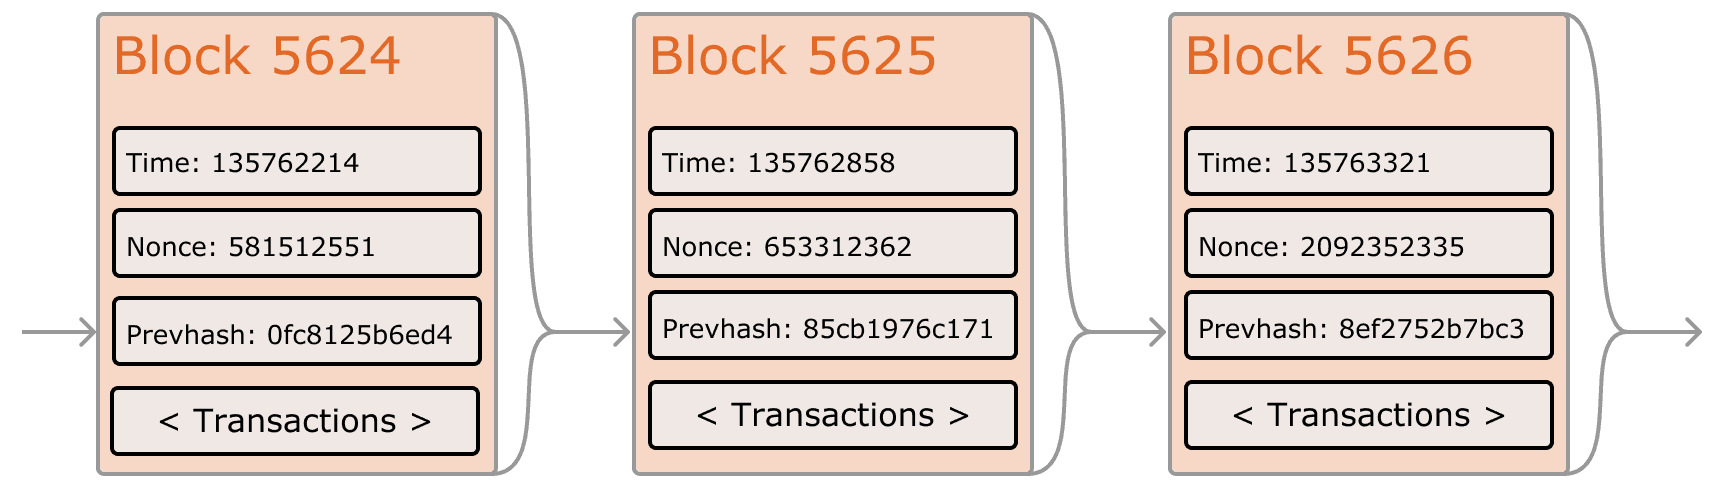
\includegraphics[width=\textwidth]{figures/ethereum-blocks.png}
        \caption{Ethereum blockchain structure.}
        \label{fig:ethereumBlockchainStructure}
    \end{figure}

    As the second most popular blockchain, the Ethereum blockchain was developed as an alternative to cover for the lackings of Bitcoin.
    It is a transaction-based, cryptographically secure state machine, that reads a series of inputs and, based on those inputs, transitions to a new state.~\cite{ferreira2022smart}
    It is a distribued ledger that supports Turing-complete programming languages, giving its users the power to write and store Turing-complete programs and define and transition between states with those programs.

    Just like Bitcoin, Ethereum currently uses Proof-of-Work (PoW) as its consensus protocol.
    Proof-of-Stake (PoS), PBFT(Practical Byzantine Fault Tolerance), and DPoS (Delegated Proof of Stake) are other forms of concensus protocol, for example.
    The solution to a series of cryptographic puzzles are used in the PoW mechanism to prove the credibility of the data being written on the blockchain, using such mechanism as their consensus protocol.
    The puzzle is usually a computationally hard but easily verifiable mathematical problem.
    When a node creates a block, it must resolve a PoW puzzle and spend computing power to achieve so. The nodes compete o=with each other over this objective function and the node with the most computing power usually succeeds ind doing so.
    After the PoW puzzle is resolved, it will be broadcasted to other nodes, so as to achieve the purpose of consensus and append a new block to the blockchain.
    It acts as a “proof” that a node has done “work” by spending its computational resources.
    This process is known as mining and nodes which decide to participate in this process and try to create new blocks are known as miners.

    As participating nodes are allowed to propose new blocks simaltaneously and at nearly the same time, it can be the case that two or more blocks are proposed at once with a valid
    hash while referencing the same parent block.
    This is called a "fork" in the blockchain nomenclature.
    Blockchain forks pose a serious issue to Ethereum.
    They result in multiple concurrent states and make it difficult for the nodes to come to an agreement concerning which state should be the correct state.
    For example, if the states were to diverge, a user might own 100 coins on one chain, 200 on another, and 300 on another.
    Forks can happen intentionally or be deliberately orchestrated.
    To prevent multiple states and help determine which fork is the most valid one, Ethereum blockchain uses a technique known as the Greedy Heaviest Observed Subtree (GHOST) protocol.
    The GHOST protocol declares that of all the states, one must select the state that contains the most computation.
    One way to determine the heaviest state (computation-wise), is to look at the block number of the most recent block (i.e., leaf block) of a state, which amounts to the total
    number of blocks in the current state (not including the genesis block).
    The higher the block number, the longer the chain of that state and the greater the mining computation that must have gone into arriving at that current leaf block.
    This allows the blockchain nodes to agree on an accpeted version of the current state of the blockchain.
    Those blocks that are not included in the canonical chain are often referred to as orphans or uncle blocks.
    Unlike other blockchains, such as Bitcoin, Ethereum also adds uncle blocks to the aforementioned calculation to figure out the longest and computationally heaviest chain of blocks.
    This allows for the inclusion of more transactions and attributes a reward to the creators of uncle blocks as well as miners for declaring concurrent blocks as uncles and
    thereby keeping forked chains as short as possible.

    \begin{figure}
        \centering
        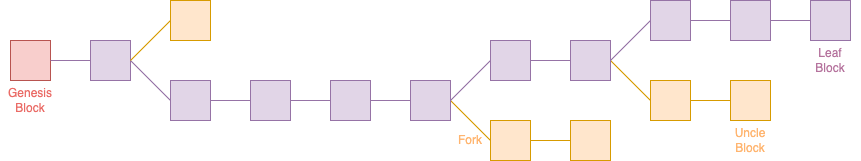
\includegraphics[width=\textwidth]{figures/uncle.png}
        \caption{An illustration of Ethereum's GHOST protocol.}
        \label{fig:uncle}
    \end{figure}

    \subsection{Ether}
        Ether is the native cryptocurrency of Ethereum.
        A cryptocurrency is a digital currency that is secured by means of cryptographic primitives.
        The purpose of ether is not only to allow users to exchange value between one another, but also to provide an economic incentive for users of its underlying platform to
        provide computational resources to the Ethereum network.
        Any network participant who sends a transactions must offer some amount of ether to the Ethereum network as a fee.
        This remuneration will be awarded to whoever gets to mine the block that includes the transaction, as a result of doing the work of verifying, executing, and broadcasting
        the transaction to the rest of the blockchain network.
        The amount of ether offered in such transaction as the corresponding fee, must correspond to the time and effort spent in executing the transaction.
        These costs prevent malicious participants from intentionally blocking up the network by requesting the execution of infinite computation or other resource-intensive actions,
        as these ill-intentioned participants must pay for the computation.

        Ethereum provides a metric system of denominations to describe different units of ether.
        Each denomination has its own unique name.
        Wei and Gwei are the most popular denominations.
        Wei is the smallest possible denomination of ether also known as the base unit, and as a result, many technical implementations base all their calculations in wei.
        Gwei (short for gigawei) is often used to describe costs related to “gas”.

    \subsection{Accounts}
        The Ethereum state is consisted of many small objects naemd as accounts, where each account has a 20-byte address and state transitions to be able to interact with the other accounts on-chain.
        An address on the Ethereum blockchain is a 160-bit identifier that is used to identify any account.
        The world state is a mapping between addresses and account states.~\cite{wood2014ethereum}
        Ethereum suppotrs two types of accounts: externally owned
        (controlled by private keys) -namely EOA's- and contract accounts (CA'S, controlled by their contract code)~\cite{ethereum2014ethereum}.
        Inside of an Ethereum account is composed of four fields: nonce, ether balance, contract code hash, and storage root, explained as follows:

        \begin{itemize}
            \item \textbf{Nonce:} Nonce represents the number of transactions sent from particular address or the number of contract creations made by an account and is used as a guarantee that each transaction can only be processed once.
            \item \textbf{Balance:} Ether balance is the number of Wei owned by this address
                Wei is the smallest subunit of ether (1 wei is equivalent to 10-18 ether).
            \item \textbf{Storage Root:} Storage root is the 256-bit hash of the root node of a Merkle Patricia tree that represents the content of the account 
            \item \textbf{Contract CodeHash:} Contract code hash is the Keccak-256 hash of Ethereum Virtual Machine (EVM) code of the account, which is executed if an address receives a message call.
        \end{itemize}

    \subsection{Transactions}
        Transactions are essentially cryptographically signed instructions from EOAs to update the state of the Ethereum blockchain.
        EOAs sign their transactions using their private key in order to cryptographically prove that the transaction could only have come from them and not from someone else.
        Two types of transactions exist: message calls and contract creations.
        The latter are transactions with an empty recipient field that result in creating new CAs (i.e., smart contracts). 
        The code, to be associated with the CA, is placed inside the data field of the transaction.
        Regardless of their type, all transactions contain the following fields:
            \begin{itemize}
                \item A count on the number of transactions sent by the sender. This number is incremented by one every time a transaction is sent by the sender.
                \item The amount of wei that the sender is willing to pay for each unit of gas that is used during the execution of the transaction.
                \item The maximum amount of gas units that the sender is willing to spent for the execution of this transaction.
                    This amount is set and paid upfront, before any computation is performed.
                \item The address of the recipient. If the recipient is an EOA, the transaction will transfer value, if the recipient is a CA, the transaction will transfer value as well as
                execute the contract's code.
                    A transaction with an empty recipient address is used to trigger the creation of a new CA.
                \item The amount of wei to be sent from the sender account to the recipient account.
                    Interestingly, this value may be used to set the starting balance of the newly created CA in a contract-creating transaction.
                \item These values represent the digital signature (R, S) which can be used to recover the public key (V).
                    These values identify the sender of the transaction and confirms that the sender has authorized the transaction.
                \item This field is only part of contract-creating transactions and consists of an unlimited length byte array that includes the code to be used during the initialization process
                and the code to be permanently associated with the newly created CA.
                \item This is an optional field that is only part of message calls and consists of a byte array of unlimited size that specifies the input data (e.g., , function name, function parameters)
                of the message call.
            \end{itemize}
            As previously mentioned, contract-creating transactions and message calls are always initiated by EOAs.
            However, this does not mean that CAs cannot communicate with other CAs.
            CAs can send messages or so-called “internal transactions” to other CAs.
            Internal transactions are similar to normal transactions, with the major difference being that they are not initiated by EOAs, but instead they are initiated by CAs.
            Moreover, internal transactions merely exist as virtual objects that, unlike transactions, are not persisted in the Ethereum blockchain and only exist at execution time.
            When a CA sends an internal transaction to another CA, the code that is associated with the recipient CA is executed.
            In contrast to normal transaction, internal transactions do not contain a gas limit by default.
            They are only limited by the gas limit that was determined by the normal transaction that triggered them.
            Thus, the gas limit that the EOA provides within its normal transaction, must be large enough to perform the execution of the normal transaction, including any sub-executions that occur
            as a result of that transaction, such as any internal transactions.
            If the execution of an internal transaction runs out of gas, then its execution will be will be reverted, along with any subsequent internal transactions triggered by the execution.
            However, the parent execution is not reverted.

    \subsection{Blocks}
        Every Blockchain, including Ethereum, consists of a sequence of blocks, which are bound and "chained" together through cryptographic hashes, grouping transactions altogether.
        A block on the Ethereum blockchain consists of a body and a header.
        The block header contains metadata about its own specific block. 
        The first block of the Blockchain is called genesis which has no parent block.
        An ommer is a block whose parent is equal to the current block's parent's parent.
        A block header is a portion of the block consisting of the following apart from the transactions listed inside:

        \begin{itemize}
            \item \textbf{ParentHash}: This is the Keccak-256 hash of the parent block's header.
            \item \textbf{OmmersHash}:This is the Keccak-256 hash of the ommer's list portion of this block.
            \item \textbf{Beneficiary}: The account address that receives the fees for mining this block
            \item \textbf{LogsBloom}: A Bloom filter (i.e., a data structure) that allows efficient querying of information contained in the logs.
            \item \textbf{Difficulty}: the diKculty level of this block, i.e. the required effort for mine a block.
            \item \textbf{Number}:  the count of current block (the genesis block has a block
            number of zero; the block number increases by 1 for each each
            subsequent block)
            \item \textbf{GasLimit}: The current gas limit per block.
            \item \textbf{GasUsed}: the sum of the total gas used by transactions in this block.
            \item \textbf{ExtraData}: Arbitrary data that can set by the miner. This data is limited to 32-byte and usually refers to the name of the miner or the client version that was used to
            mine the block.
            \item \textbf{StateRoot}: the hash of the root node of the state trie (recall how we
            learned that the state trie is stored in the header and makes it easy
            for light clients to verify anything about the state)
            \item \textbf{Timestamp}: The UNIX timestamp when the block was mined.
            \item \textbf{Nonce}: A hash that, when combined with the mixHash, proves that this block has carried out enough computation
            \item \textbf{MixHash}: A hash that, when combined with the nonce, proves that
            this block has carried out enough computation
            \item \textbf{TransactionsRoot}: The hash of the root node of the Merkle Patricia trie that stores all transactions listed in this block.
            \item \textbf{ReceiptsRoot}: The hash of the root node of the Merkle Patricia trie that stores the receipts of all transactions listed in this block.
                Transaction receipts are generated after the execution of a transaction contain information such as logs or the actual gas that has been used during execution.

        \end{itemize}

    \subsection{Ethereum Virtual Machine}
        
        The Ethereum Virtual Machine (EVM) at the heart of the Ethereum blockchain is a VM (virtual machine), with a stack-based architecture, supporting Turing-complete programming languages.
        It is basiaclly the compute system in Ethereum for the execution of smart contracts, and usually dubbed as the OS of the Ethereum.
        For a simple analogy, you can think if it like the Java programming langauge that uses the Java Virtual Machine (JVM).
        Wood actually introduces EVM as a quasi-Turning-complete machine, as they state that computation is fundamentally bounded in Ethereum through the introdution of the concept of gas comnsuption.
        The word size of the machine (and thus size of stack item) is 256-bit.
        This was chosen to facilitate the Keccak256 hash scheme and elliptic-curve computations.
        The memory model is a simple word-addressed byte array.
        The stack has a maximum size of 1024.
        The machine also has an independent storage model;
        this is similar in concept to the memory but rather than a byte array, it is a wordaddressable word array.
        Unlike memory, which is volatile, storage is non volatile and is maintained as part of the system state.
        All locations in both storage and memory are well-defined initially as zero.


\section{Smart Contracts}
    The concept of smart contracts - programs running on the EVM - has been first introduced by Nick Szabo in one of his works in 1997.~\cite{szabo1997formalizing}

    \subsection{Vulnerabilities}
        Solidity, like any other programming langauge in history, is prone to all kinds of vulnreabilities.
        What makes security vulnerabilities in Solidity so attractive is the fact that the programs written in Solidity are very much often used in the financial sector, handling millions of dollars in digital aassets and cryptocurrencies.


            \paragraph{Re-entrancy}
                

            \paragraph{Access Control}
                

            \paragraph{Frontrunning}
                

            \paragraph{Bad Randomness}
            Also known as \textit{nothing is secret},~\cite{dasp} this vulnerability happens when smart contracts attempt to generate random, or to be more exact, pseudo-random numbers for any number of reasons.
            If the smart contract generating the pseudo-random number computes that random number using values that can be guessed by a malicious party, then the attacker can predict the next number that will be generated.
            Values such as block timestamps,or block number are generally advised against to be used in such mechanisms. They are called hard-to-predict values but it is better to use an external oracle to generate the random numbers needed~\cite{swcregistry}.

                
        
            \paragraph{Time Manipulation}
                
        
            \paragraph{Short Address}
                
